\documentclass[arbeit=studie,oneside,BCOR=12mm]{ArbeitRST}
% Die Option BCOR legt den Rand für die Bindekorrektur links fest
% (verschiebt das ganze Dokument nach rechts auf dem Papier, damit
% Platz zum Binden ist

% bib-Datei mit den Literaturangaben
% ==================================
\addbibresource{Literatur-Arbeit.bib}

% Paket zum Erzeugen von Blindtext 
% ================================
% (ist nur für dieses Beispieldokument sinnvoll)
\usepackage{blindtext}
\usepackage{physics}
\usepackage{amsmath}


% Zwei Parameter zum Verändern des Layouts
% ========================================
% \parindent -> Legt fest, mit welcher Einrückung jeder neue
%               Absatz beginnen soll
% \parskip -> Legt fest, wieviel vertikaler Abstand zwischen zwei
%             Absätzen liegen soll
%
% Tipp: Entweder parindent auf Null und parskip auf einen Wert
% ungleich Null (z.B. 2ex) oder umgekehrt. Beide Werte ungleich
% Null macht satztechnisch keinen Sinn. 1ex = Breite des 
% Buchstabens x
\setlength{\parindent}{0ex}
\setlength{\parskip}{2ex}



% Einige Einstellungen für das hyperref-Paket
% =========================================== 
% Hiermit können Links, Gleichungsnummern etc. farbig dargestellt
% werden was die Navigation im elektronischen Dokument vereinfacht. An
% dieser Stelle können Sie die Farbgebung anpassen. Druckversion bitte
% ohne farbige Links erstellen, siehe Option unten!
\hypersetup{
    unicode=false,          % non-Latin characters in Acrobat’s bookmarks
    pdftoolbar=true,        % show Acrobat’s toolbar?
    pdfmenubar=true,        % show Acrobat’s menu?
    pdffitwindow=false,     % window fit to page when opened
    pdfstartview={FitH},    % fits the width of the page to the window
    pdftitle={RST Vorlage}, % title
    pdfauthor={Author},     % author
    pdfsubject={Subject},   % subject of the document
    pdfcreator={Creator},   % creator of the document
    pdfproducer={Producer}, % producer of the document
    pdfkeywords={keyword1} {key2} {key3}, % list of keywords
    pdfnewwindow=true,      % links in new window
    colorlinks=true,        % false: boxed links; true: colored links
    linkcolor=blue,         % color of internal links (change box color with linkbordercolor)
    citecolor=green,        % color of links to bibliography
    filecolor=magenta,      % color of file links
    urlcolor=cyan           % color of external links
}

% Entfernt die farbigen Markierungen - bitte Druckversion mit dieser Option kompilieren
%\hypersetup{hidelinks}

   

% =================================================================
\begin{document}

% Titelseite
% ==========

% Name des Verfassers
\author{Julius Fiedler}

% Geburtsort
\geburtsort{Dresden}

% Geburtsdatum
\geburtsdatum{13. Oktober 1996}

% Titel der Arbeit
\title{Über den Einfluss hochfrequenter mechanischer Oszillationen auf das Schaltverhalten supraleitender PID-Regler auf Quantenbasis}

% Untertitel
\subtitle{Eine Fallstudie unter besonderer Berücksichtigung stochastischer Einflüsse}

% Angabe der Betreuer
\betreuer{Betreuer 1}
\betreuer{Betreuer 2}

% Datum der Einreichung
\date{2. Februar 2222}


% Zunächst für das Vorgeplänkel römische Seitenzahlen und einfacher Seitenstil
% ============================================================================
\pagenumbering{Roman}
\pagestyle{plain}


% Titelseite erstellen
\maketitle


% Selbstständigkeitserklärung
% ===========================

% Ort der Selbstständigkeitserklärung (Standard: Dresden)
\selbstort{Pirna}

% Datum der Selbstständigkeitserklärung (Standard: aktuelles Systemdatum)
\selbstdatum{1. Januar 2016}

% Selbstständigkeitserklärung erstellen
\selbststaendigkeitserklaerung


% Kurzfassung / Abstract
% ======================
\kurzfassung{An dieser Stelle fügen Sie bitte eine deutsche Kurzfassung ein.}{Please insert the English abstract here.}


% Inhaltsverzeichnis
% ==================
\tableofcontents

% Ggf. Symbolverzeichnis
% ======================
\chapter*{Verzeichnis der Formelzeichen \markboth{VERZEICHNIS DER FORMELZEICHEN}{}} \label{ch:Symbolverzeichnis}
\addcontentsline{toc}{chapter}{Verzeichnis der Formelzeichen}

\begin{table}[htbp]
\centering
\begin{tabular}{llp{9 cm}}
$C^r(n,k)$ & Kombination mit Wiederholung
$\varepsilon$ & Fehler der Moore-Penrose-Lösung\\
$\varepsilon_\text{r}$& relativer Fehler der identifizieren Koeffizienten\\
$\boldsymbol{f}$ & Systemdynamik\\
$F$ & Kraft, die auf den Wagen wirkt\\
$g$ & Erdbeschleunigung\\
$m$ & Anzahl der Messungen\\
$m_1$ & Masse des Wagens\\
$m_2$ & Masse am Ende des Pendels\\
$n$ & Anzahl der Zustände\\
$L$ & Anzahl der Ansatzfunktionen in $\Theta$\\
$\boldsymbol{p}$ & Parametervektor\\
$P$ & nominale Koeffizientenmatrix\\
$\varphi$ & Auslenkung des Pendels aus der unteren Ruhelage\\
$Q$ & identifizierte Koeffizientenmatrix\\ 
$R$ & Hilfsmatrix zur Berechnung von $\varepsilon_\text{r}$\\
$s$ & Länge des Pendels\\
$t$ & Zeit \\
$\theta$ & Gruppe von Ansatzfunktionen\\
$\Theta$ & $\Theta(X)$\\
$\Theta(X)$ & Bibliotheksmatrix aus Ansatzfunktionen, ausgewertet für alle von $X$\\
$\Theta^+$ & Moore-Penrose-Inverse von $\Theta$\\
$\Theta_\text{v}$ & verkleinerte Bibliotheksmatrix\\
$U$ & Unbekannte Funktion\\
$x$ & Position des Wagens\\
$\boldsymbol{x}(t)\in\mathbb{R}^n$ & Zustandsvektor\\
$X$ & Matrix der zeitlichen Verläufe der Zustandskomponenten\\
$\dot{X}$ & Matrix der zeitlichen Verläufe der Ableitungen der Zustandskomponenten\\
$\xi$ & Spalte von $\Xi$\\
$\Xi$ & Koeffizientenmatrix\\
$\Xi^\text{d}$ & dünn besetzte Koeffizientenmatrix\\
$\hat{\Xi}$ & verkleinerte Koeffizientenmatrix unter Nutzung von $\Theta_\text{v}$\\
$\Xi^n$ & Koeffizientenmatrix in den Dimensionen von $\Xi$ mit den Einträgen von $\hat{\Xi}$\\

\end{tabular}
\end{table}

% Ggf. Abbildungsverzeichnis
% ==========================
\listoffigures


% Ggf. Tabellenverzeichnis
% ========================
\listoftables


% ========================
% Beginn Inhalt der Arbeit
% ========================

% Inhalt kann entweder in separate LaTeX-Dateien ausgelagert werden
% (hier: inhalt.tex) und dann mittels \input{} geladen werden...
% Darauf achten, dass pagenumbering und pagestyle richtig gesetzt werden
% (siehe Einträge in inhalt.tex)


%\chapter{Erläuterungen zur Klasse ArbeitRST}

% Ab hier arabische Seitenzählung und heading Seitenstil
\pagestyle{scrheadings}
\pagenumbering{arabic}

In den folgenden Abschnitten werden einige Erläuterungen zur \LaTeX-Dokumentenklasse \texttt{ArbeitRST.cls} gegeben werden. Diese basiert auf der Klasse \texttt{scrbook} aus dem KOMA-Script-Paket und kann daher mit Hilfe der Methoden aus diesem Paket modifiziert werden. Für nähere Informationen dazu sei auf die KOMA-Script-Anleitung\footnote{Diese kann unter der URL \url{http://www.ctan.org/pkg/koma-script} heruntergeladen werden.} und die Website
\begin{center}
	\url{http://www.komascript.de/}
\end{center}
verwiesen. 

Die wesentlichsten Änderungen gegenüber der ursprünglichen Klasse bestehen in einer angepassten Titelseite und der hinzugefügten Selbstständigkeitserklärung.



% ====================================================
\section{Informationen zu schriftlichen Arbeiten am RST}
Informieren Sie sich in der für Sie relevanten Prüfungsordnung über die \emph{Anzahl der geforderten Exemplare} die eingereicht werden müssen. Bitte beachten Sie, dass jedes dieser Exemplar die \emph{Aufgabenstellung} enthalten muss. Lassen Sie diese bitte beim Binden zwischen der Titelseite und der Selbstständigkeitserklärung einfügen. Eines der Exemplare muss dabei das \emph{originale}, vom Vorsitzenden des Prüfungsausschusses und dem verantwortlichen Hochschullehrer unterzeichnete, Dokument enthalten, bei den restlichen genügen Kopien. Bitte beachten Sie, dass die Arbeit \emph{einseitig} ausgedruckt werden muss. Ausschlaggebend für die fristgemäße Einreichung ist die \emph{Bestätigung des Prüfungsamtes}. Informieren Sie sich daher im \emph{Vorfeld} über die Öffnungszeiten am Abgabetag. Sollte das Prüfungsamt geschlossen haben, ist es in der Regel möglich mit den Mitarbeitern eine individuelle Vereinbarung zu treffen.


% ====================================================
\section{Die Titelseite}
Die Titelseite kann über die in Tabelle \ref{tab:titel} angegebenen Befehle angepasst werden.
\begin{table}[htbp]
\caption{Befehle zum Anpassen der Titelseite}
\label{tab:titel}
\begin{tabular}{lp{12cm}}
Befehl & Bedeutung\\
\toprule
\verb|\author| & legt den Namen des Autors der Arbeit fest\\
\verb|\geburtsdatum| & legt das Geburtsdatum des Autors fest\\
\verb|\geburtsort| & legt das Geburtsort des Autors fest\\
\verb|\title| & legt den Titel der Arbeit fest\\
\verb|\subtitle| & legt den Untertitel der Arbeit fest\\
\verb|\betreuer| & fügt einen Betreuer hinzu\\
\verb|\date| & legt das Einreichungsdatum der Arbeit fest -- \newline wird dieser Befehl nicht aufgerufen wird standardmäßig das zum Kompilationszeitpunkt eingestellte Systemdatum verwendet.\\
\bottomrule
\end{tabular}
\end{table}



% ====================================================
\section{Die Selbstständigkeitserklärung}
In der Selbstständigkeitserklärung werden automatisch der Typ der Arbeit, ihr Titel sowie der Name des Autors übernommen. Der Ort kann über den Befehl \verb|\selbstort| geändert werden, wobei standardmäßig "`Dresden"' verwendet wird. Das Datum ist standardmäßig identisch zum Einreichungsdatum, kann aber mit dem Befehl \verb|\selbstdatum| geändert werden.



% ====================================================
\section{Kurzfassung}
Eine Kurzfassung der Arbeit kann mit dem Befehl \verb|\kurzfassung{deutsch}{englisch}| eingefügt werden. Das erste Argument entspricht dabei der deutschen, das zweite der englischen Version.



% ====================================================
\section{Auswahl des Typs der Arbeit}
Zur Auswahl des Typs der Arbeit steht die Klassenoption \texttt{arbeit} zur Verfügung. Mit dieser können sie zwischen Diplom-, Master- und Studienarbeit sowie dem Bericht zum Forschungspraktikum auswählen:
\begin{table}[hbtp]%
\caption{Auswahl des Typs der Arbeit mittels Klassenoptionen}
\centering
\begin{tabular}{cc}
Diplomarbeit & \verb|\documentclass[arbeit=diplom]{ArbeitRST}|\\
Masterarbeit & \verb|\documentclass[arbeit=master]{ArbeitRST}|\\
Studienarbeit & \verb|\documentclass[arbeit=studie]{ArbeitRST}|\\
Bericht zum Forschungspraktikum & \verb|\documentclass[arbeit=forsch]{ArbeitRST}|
\end{tabular}
\label{}
\end{table}



% ====================================================
\section{Eingebundene Pakete}
In der Dokumentenklasse werden bereits einige \LaTeX-Pakete geladenen. Davon sind die zum Verfassen einer Arbeit möglicherweise relevanten in der Tabelle \ref{tab:pakete} aufgeführt. 
\begin{table}[htbp]%
\centering
\caption{Auswahl eingebundener Pakete}
\label{tab:pakete}
\begin{tabular}{p{3.6cm}p{11.4cm}}
amsmath, amssymb, \newline amsfonts, amsthm & Pakete zum Satz mathematischer Formeln, Dokumentation finden sie unter \newline\url{http://www.ams.org/publications/authors/tex/amslatex},\newline besonders empfehlenswert ist der "`Short Math Guide for \LaTeX"'\\
booktabs & ermöglicht das Setzen "`schöner"' Tabellen, Dokumentation unter \url{http://ctan.org/pkg/booktabs}\\
cite & verbessert einige Aspekte des Zitierens, Dokumentation unter \newline\url{http://ctan.org/pkg/cite}\\
caption, subcaption & Pakete zum Anpassen der Unter- und Überschriften von Tabellen, Grafiken etc., Dokumentation unter \newline\url{http://ctan.org/pkg/caption} \newline\url{http://ctan.org/pkg/subcaption}
\end{tabular}
\end{table}\\
Neben diesen Paketen wird das Paket \verb|hyperref| (\url{http://ctan.org/pkg/hyperref}) zur farbigen Hervorhebung von Verweisen, Links etc.\ eingebunden. Bitte deaktivieren Sie diese Markierungen vor dem Ausdrucken mit Hilfe des Befehls
\begin{center}
\verb|\hypersetup{hidelinks}|.
\end{center}



% ====================================================
\section{Zusätzliche Makros}
In die Dokumentenklasse \texttt{ArbeitRST} wurden einige Makros aufgenommen, die sich bei der Arbeit mit \LaTeX{} als nützlich erwiesen haben.
\begin{table}[htbp]
\centering
\caption{Zusätzliche Makros und Umgebungen}
\begin{tabular}{ccp{9cm}}
Syntax & Ausgabe & Beschreibung\\
\toprule
\texttt{\textbackslash vect\{a\}} & $\vect{a}$ & Umschaltung auf fette Schriftart im Mathemodus-- oft für Vektoren genutzt\\[2ex]
\texttt{\textbackslash diag(a,\textbackslash ldots,z)} & $\diag(a,\ldots,z)$ & Nützlich zur Definition von Diagonalmatrizen\\[2ex]
\texttt{\textbackslash diff[n]\{q\}\{t\}} & $\diff[n]{q}{t}$ & Ableitungen darstellen\\[2ex]
\texttt{\textbackslash partiell[n]\{q\}\{t\}} & $\partiell[n]{q}{t}$ & partielle Ableitungen darstellen\\[2ex]
\texttt{\textbackslash dr} &$\dr$ &Aufrechtes d für Integrale ($\int f(t) \dr t$)\\[2ex]
\texttt{\textbackslash Reals} & $\Reals$ & Körper der reellen Zahlen\\[2ex]
\texttt{\textbackslash Compl} & $\Compl$ & Körper der komplexen Zahlen\\[2ex]
\texttt{\textbackslash Real(a)} & $\Real(a)$ & Realteil von $a$\\[2ex]
\texttt{\textbackslash Imag(a)} & $\Imag(a)$ & Imaginärteil von $a$\\[2ex]
\texttt{\textbackslash norm\{a\}} & $\norm{a}$ & Norm von $a$\\[2ex]
\texttt{\textbackslash abs\{a\}} & $\abs{a}$ & Betrag von $a$\\[2ex]
\texttt{\textbackslash skalprod\{a\}\{b\}} & $\skalprod{a}{b}$ & Skalarprodukt von $a$ und $b$\\[2ex]
\texttt{\textbackslash grad(a)} & $\grad(a)$ & Gradient von $a$\\[2ex]
\texttt{\textbackslash div(a)} & $\div(a)$ & Divergenz von $a$\\
\bottomrule
\end{tabular}
\end{table}


Neben diesen Makros wurden Umgebungen zum Erzeugen von Definitionen (\verb|definition|), Beispielen (\verb|beispiel|), Lemmata (\verb|lemma|) und Bemerkungen (\verb|bemerkung|) definiert.

\begin{table}[htbp]%
\centering
\caption{Beispiele der vordefinierten Umgebungen}
\begin{tabular}{p{8cm}p{7cm}}
Syntax & Ausgabe\\
\toprule
\begin{verbatim}
\begin{definition}[Beispiel]
Beispiel für eine Definitionsumgebung
\end{definition}
\end{verbatim}
&
\begin{definition}[Beispiel]
Beispiel für eine Definitionsumgebung
\end{definition}
\\
\begin{verbatim}
\begin{beispiel}[Beispiel]
Beispiel für eine Beispielumgebung
\end{beispiel}
\end{verbatim}
&
\begin{beispiel}[Beispiel]
Beispiel für eine Beispielumgebung
\end{beispiel}
\\
\begin{verbatim}
\begin{lemma}[Beispiel]
Beispiel für eine Lemmaumgebung
\end{lemma}
\end{verbatim}
&
\begin{lemma}[Beispiel]
Beispiel für eine Lemmaumgebung
\end{lemma}
\\
\begin{verbatim}
\begin{bemerkung}[Beispiel]
Beispiel für eine Bemerkungsumgebung
\end{bemerkung}
\end{verbatim}
&
\begin{bemerkung}[Beispiel]
Beispiel für eine Bemerkungsumgebung
\end{bemerkung}\\
\bottomrule
\end{tabular}
\end{table}



% ====================================================
\section{Weitere Informationen}
Da \LaTeX\ seine Funktionalität im wesentlichen durch frei verfügbare Pakete erhält, ist es günstig eine Distribution zu installieren, die bereits die wesentlichen Pakete enthält und das Hinzufügen weiterer Pakete vereinfacht. Für Windows existiert beispielsweise MiKTeX (\url{http://miktex.org/}) und für Linux TeX Live (\url{http://www.tug.org/texlive/}). Zum Erstellen von \LaTeX-Dokumenten unter Windows hat sich das Programm TeXnicCenter (\url{http://www.texniccenter.org/}), vor allem in Verbindung mit dem Sumatra PDF-Betrachter (\url{http://blog.kowalczyk.info/software/sumatrapdf}), als sehr nützlich erwiesen. Unter Linux gilt dasselbe für das Programm Kile (\url{http://kile.sourceforge.net/}). Zum Erstellen und Verwalten von Bibtex-Dateien wurden gute Erfahrungen mit JabRef (\url{http://jabref.sourceforge.net/}) gemacht. Es existieren zahlreiche Bücher zum Umgang mit \LaTeX, von denen an dieser Stelle nur \cite{MittelbachGoosens05} aufgeführt wird.


%%% Local Variables:
%%% mode: latex
%%% TeX-master: "ArbeitRST"
%%% End:


\pagenumbering{arabic}
% ...oder man schreibt direkt in dieser Datei (weniger übersichtlich)
\chapter{Notizen}

\section{UDE}

\begin{figure}[ht]
\begin{subfigure}[c]{0.5\textwidth}
\centering
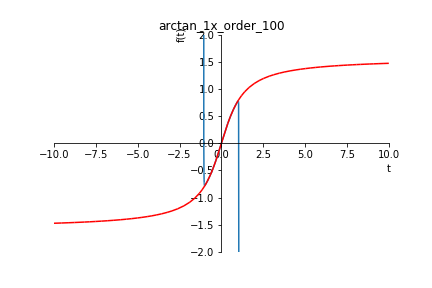
\includegraphics[width=1\textwidth]{images/arctan_1x_order_100}

\end{subfigure}
\begin{subfigure}[c]{0.5\textwidth}
\centering
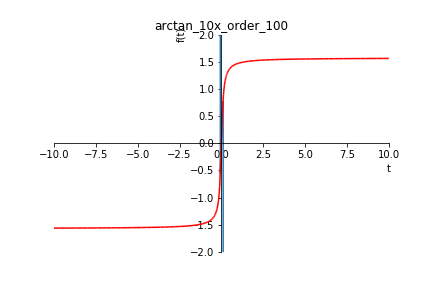
\includegraphics[width=1\textwidth]{images/arctan_10x_order_100}

\end{subfigure}
\begin{subfigure}[c]{0.5\textwidth}
\centering
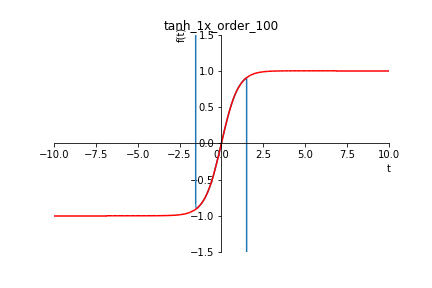
\includegraphics[width=1\textwidth]{images/tanh_1x_order_100}

\end{subfigure}
\begin{subfigure}[c]{0.5\textwidth}
\centering
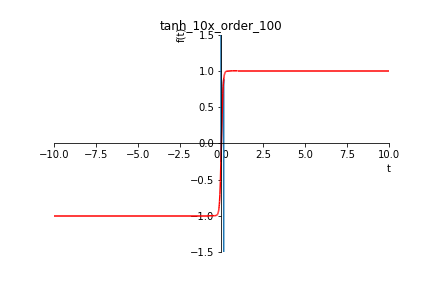
\includegraphics[width=1\textwidth]{images/tanh_10x_order_100}

\end{subfigure}
\end{figure}


\subsection{8.7.20} 
überlegung NN in julia und sindy in python machen, export erledigt\\
trotzdem keine identifikation in python möglich, grund: zu wenig daten (datenfeld mit 31 daten Autflösung viel zu gering)\\
bei erhöhung der auflösung wird trainingszeit enorm groß
NN approximiert den verlauf der ableitungen	\\
sindy mal mit anderen anfangswerten trainieren
\subsection{9.7.20}
ude keine option für multiple trajectories / threshhold???
\subsubsection{ude + sindy}
definitorische Gleichungen bekannt\\
dt=0.1\\
sindy did not converge
\begin{align}
du_1 &= cos(u_3) * p_1\\
du_2 &= sin(u_3) * p_2\\
du_3 &= sin(u_1) * p_3 + p_4 * u_1\\
du_4 &= sin(u_3) * p_5
\end{align}
parameters: Float32[0.050624948, 0.006272168, -20.755184, -13.720979, -0.01513608]
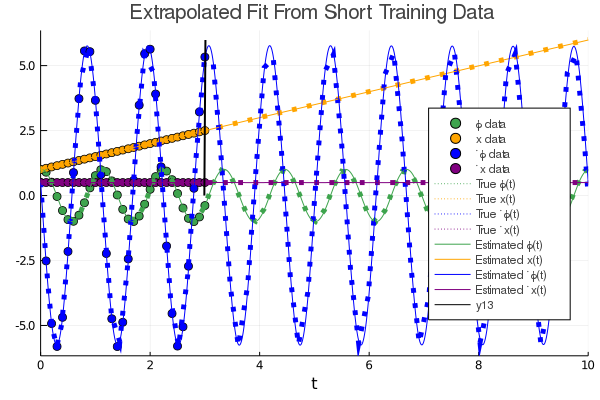
\includegraphics[width=1\textwidth]{images/ude_ident_with_prior_knowledge}
im Vergleich: nur den Sindy Part in PySindy ausgelagert ergibt: (dieser Vergleich ist nicht sinnvoll? pysindy kennt ja die def. gl nicht)
\begin{align*}
phi' &= 65170415.755 xdot + -72812822.138 sin(xdot) + 2647179.524 cos(xdot)\\
x' &= 51018334.340 xdot + -57002163.483 sin(xdot) + 2072882.755 cos(xdot)\\
phidot' &= -3.002 phi + -6.328 x + 2682545588.568 xdot + -33.032 sin(phi) \\&+ -1.358 sin(x) + -0.208 sin(phidot) + -2997205703.337 sin(xdot) \\&+ -0.020 cos(phi) + -6.583 cos(x) + 109008747.059 cos(xdot)\\
xdot' &= 0.320 x + -18300414.600 xdot + 20447317.167 sin(xdot) + 0.344 cos(x) \\&+ -743815.199 cos(xdot)
\end{align*}




keine Gleichungen bekannt\\
dt=0.1\\
sindy did not converge
\begin{align}
du_1 &= p_1 * u_3\\
du_2 &= sin(u_2) * p_2\\
du_3 &= sin(u_1) * p_3 + p_4 * u_1\\
du_4 &= cos(u_1) * p_5
\end{align}
parameters: Float32[0.997858, 0.20674846, -18.494001, -15.788721, 0.040644586]\\
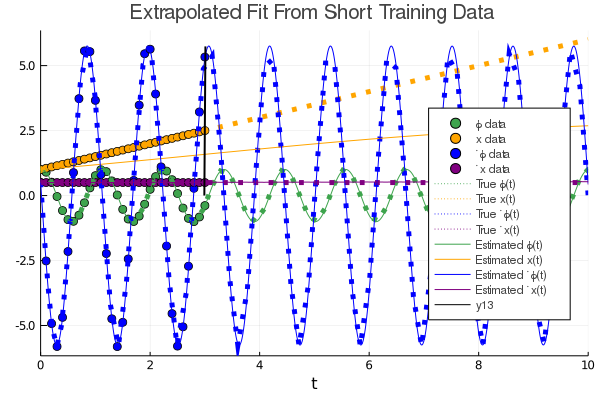
\includegraphics[width=1\textwidth]{images/ude_ident_without_prior_knowledge}
im Vergleich: nur den Sindy Part in PySindy ausgelagert ergibt:
\begin{align*}
phi' &= 1.111 phi + 0.648 x + 1.002 phidot + -503701656.178 xdot + -1.228 sin(phi) \\&+ 562779966.638 sin(xdot) + -0.050 cos(phi) + 0.676 cos(x) + -20465608.922 cos(xdot)\\
x' &= 0.833 phi + -0.031 x + 450669011.982 xdot + -0.967 sin(phi) \\&+ -503527393.951 sin(xdot) + 0.157 cos(phi) + -0.051 cos(x) + 18310968.307 cos(xdot)\\
phidot' &= -2.551 phi + -4.834 x + -3252316739.183 xdot + -33.509 sin(phi) \\&+ -0.458 sin(x) + 3633781720.861 sin(xdot) + -5.066 cos(x) + -132146405.440 cos(xdot)\\
xdot' &= 0.674 phi + -184783222.592 xdot + -0.759 sin(phi) + 206455836.816 sin(xdot) + \\&-7507657.694 cos(xdot)
\end{align*}

\subsubsection{ude reibung}
tanh wie erwartet problematisch, vmtl sinnvoll tanh vorzugeben\\
viskose+ haftreibung:
\begin{align*}
du_1 &= sin(u_3) * p_1\\
du_2 &= cos(u_1) * p_2 + cos(u_3) * p_3\\
du_3 &= p_4 * u_3\\
du_4 &= sin(u_3) * p_5
\end{align*}
parameters: Float32[-0.032978103, 0.020778582, 0.02180107, -0.30371103, -0.026243187]
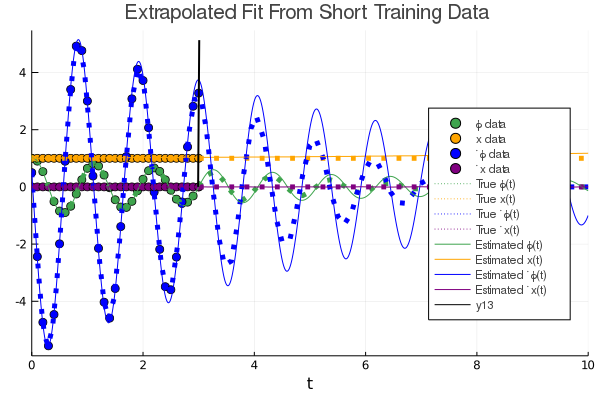
\includegraphics[width=1\textwidth]{images/ude_fric_order_4}

nur viskose reibung, order 2:\\
\begin{align*}
d_1&=0.3\\
d_{1, ident}&= 0.2981498
\end{align*}

\begin{figure}
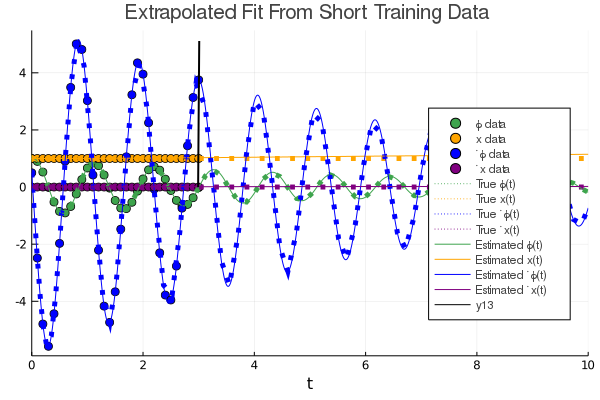
\includegraphics[width=1\textwidth]{images/ude_fric_viskos_d1_03}
\caption{ude fric viskos d1 03}
\end{figure}

viskose + haftreibung: order 1, tanh vorgegeben:\\
\begin{align*}
du_1 &= cos(u_1) * p_1\\
du_2 &= sin(u_3) * p_2\\
du_3 &= tanh(10u_3) * p_3 + p_4 * u_3\\
du_4 &= tanh(10u_3) * p_5
\end{align*}
parameters: Float32[0.018757716, -0.011911368, -0.26272112, -0.35348737, -0.005909097]

\begin{figure}
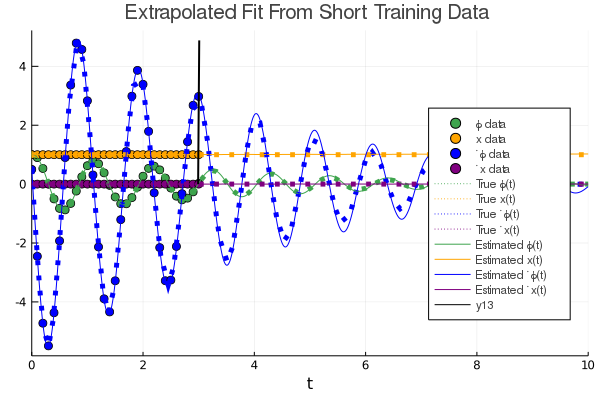
\includegraphics[width=1\textwidth]{images/ude_fric_viskos_d1_03_d2_05}
\caption{ude fric viskos und haft d1 03 d2 05}
\end{figure}


\subsubsection{Pysindy reibung}
Ansatz: Sindy für Differenz von Realem Modell mit Reibung und theoretischem Modell verwenden, siehe Bsp:\\
\begin{figure}
\begin{subfigure}[c]{0.5\textwidth}
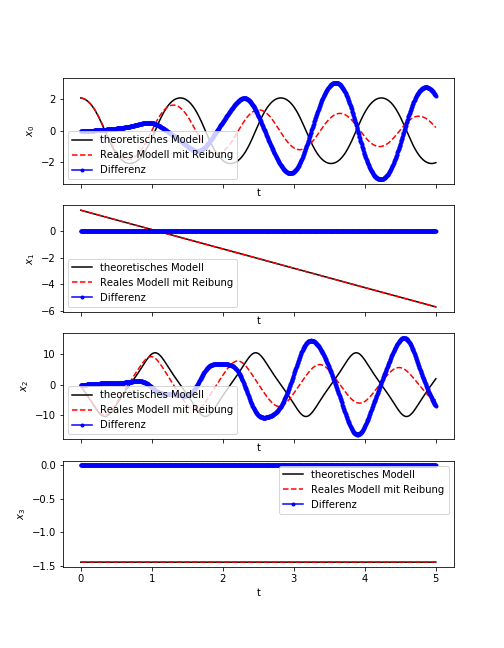
\includegraphics[width=1\textwidth]{images/pysindy_fric_visk2}
\end{subfigure}
\begin{subfigure}[c]{0.5\textwidth}
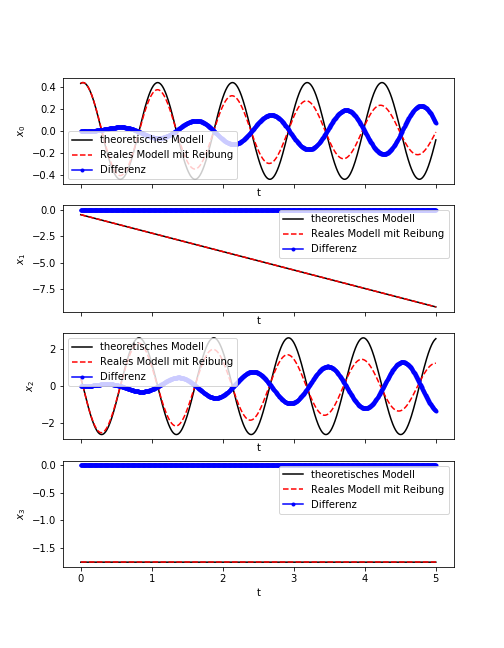
\includegraphics[width=1\textwidth]{images/pysindy_fric_visk1}
\end{subfigure}
\caption{nur viskose Reibung}
\end{figure}
keine Identifikation feststellbar\\
vermutung: aus Differenz geht keine exp funktion hervor, es fehlt die info über das vorherige System
idee: prior system knowledge integrieren indem man das bekannte teilsystem aus library funktion zur verfügung stellt
\section{Sindy}
\subsection{Funktionsweise der Methode}
Sparse Identification of Nonlinear Dynamics (SINDy) ist eine Methode, um aus Messdaten eines Systems dessen Systemdifferentialgleichungen zu schätzen.\\
Sei $x(t)\in\mathbb{R}^n$ der Zustandsvektor mit $x(t) = [x_1(t), x_2(t), ... , x_n(t)]$. Gesucht ist die Funktion der zeitlichen Ableitung des Zustandes $\dv{x(t)}{t} = f(x(t))$, welche auch nichtlinear sein kann. %d/dt gut so?
Die zugrundeliegende Überlegung der Methode ist, dass die Funktion $f$ in einem geeigneten Raum an Basisfunktionen oft \textit{dünn besetzt} ist. Betrachtet man beispielsweise die Funktion
\begin{equation}
\dv{x}{t} = f(x) = \begin{bmatrix} f_1(x)\\ f_2(x)\\ \end{bmatrix}
=\begin{bmatrix} 1+2x_1+x_1x_2^2 \\ x_1^3-3x_2\\ \end{bmatrix}
\end{equation}
so ist leicht zu erkennen, dass $f$ in Bezug auf die Basis von Polynomen aus zwei Variablen (z.B. $f_1(x)=\sum_{i=0}^{\infty}\sum_{j=0}^{\infty}a_{ij}x_1^ix_2^j$) dünn besetzt ist. Nur eine sehr geringe Zahl der Koeffizienten $a_{ij}$ ist ungleich null.
SINDy versucht nun mittels Regression diejenigen Monome auszuwählen, die die Funktion $f$ am besten repräsentieren können.\\
Für die Anwendung von SINDy benötigt man die Messdaten aller Zustandsgrößen zu den Zeitpunkten $t_1, t_2, ..., t_m)$. Zusätzlich müssen die zeitlichen Ableitungen der Zustände an den gegebenen Zeitpunkten gegeben sein, entweder durch direkte Messung oder durch numerische Approximation. Die Daten werden wie folgt angeordnet: 
\begin{align}
X &= \begin{bmatrix}
		x_1(t_1) & x_2(t_1) & \dots & x_n(t_1) \\
		x_1(t_2) & x_2(t_2) & \dots & x_n(t_2) \\
		\vdots   & \vdots   & 		& \vdots \\ 
		x_1(t_m) & x_2(t_m) & \dots & x_n(t_m)
	\end{bmatrix} \in \mathbb{R}^{m\times n},
	\\
	\dot{X} &= \begin{bmatrix} 
		\dot{x_1}(t_1) & \dot{x_2}(t_1) & \dots & \dot{x_n}(t_1) \\
		\dot{x_1}(t_2) & \dot{x_2}(t_2) & \dots & \dot{x_n}(t_2) \\
		\vdots 		   & \vdots 		& 		& \vdots \\
		\dot{x_1}(t_m) & \dot{x_2}(t_m) & \dots & \dot{x_n}(t_m)
	\end{bmatrix}  \in \mathbb{R}^{m\times n}.
\end{align}
Nun muss man die Bibliothek $\Theta$ an Funktionen konstruieren, durch welche $f$ dargestellt werden soll. Hier ist es günstig, wenn man bereits weiß, welche Funktionsklassen in $f$ vorkommen, um die Bibliothek geeignet auszulegen.
Die Spalten der Bibliotheksmatrix repräsentieren die gewählten Ansatzfunktionen, angewendet auf die Datenmatrix $X$ 
\begin{equation}
\Theta(X) = \begin{bmatrix}
		\mid & \mid & & \mid \\
		\theta_1(X) & \theta_2(X) & \dots & \theta_\ell(X) \\
		\mid & \mid & & \mid 
	\end{bmatrix}\in\mathbb{R}^{m\times L}.
\end{equation} 
Wählt man beispielsweise für $\theta_1$ die Sinusfunktion und für $\theta_2$ Monome zweiten Grades so ergeben sich 
\begin{align}
\theta_1(X) &= \begin{bmatrix}
		\mid 	  & \mid     		  &          & \mid             \\
		\sin(x_1(t)) & \sin(x_2(t))   & \dots    & \sin(x_n(t)) \\
		\mid      & \mid     		  &          & \mid              
	\end{bmatrix},\\
\theta_2(X) &= \begin{bmatrix}
		\mid & \mid & & \mid & \mid & & \mid \\
		x_1(t)^2 & x_1(t)x_2(t) & \dots & x_2(t)^2 & x_2(t)x_3(t) & \dots & x_n^2(t) \\
		\mid & \mid & & \mid & \mid & & \mid
	\end{bmatrix},	
\end{align}
wobei die Rechenoperationen alle elementweise zu lesen sind. \\
Gesucht sind nun Linearkombinationen von Bibliotheksfunktionen, sodass gilt
\begin{equation}
f_i(x) = \Theta(x^T)\xi_i.
\end{equation}
Fasst man alle $\xi_i$ in eine Koeffizientenmatrix $\Xi\in\mathbb{R}^{L\times n}$ zusammen, so ergibt sich das zu lösende Problem zu 
\begin{equation}
\dot{X} \approx \Theta(X)\Xi.
\end{equation}
In der Praxis sollte dieses Gleichungssystem überbestimmt sein. Das bedeutet, dass die Anzahl der Messzeitpunkte $m$ (die Anzahl der Zeilen) größer ist als die Anzahl der Einträge in $\Xi\in\mathbb{R}^{L\times n}$ (Anzahl der Unbekannten). Um das SINDy-Problem zu lösen, wird die Methode der kleinsten Quadrate angewendet. Durch aufstellen der Pseudo-Inversen ergibt sich 
\begin{equation}
\Xi = \left(\Theta(X)^T\Theta(X)\right)^{-1}\Theta(X)^T\dot{X} %stimmt das  auch für Matrizen?
\end{equation}
Im Programm implementiert: mit
\begin{equation}
\Xi_\text{neu} = \left(\Theta(X)^T\Theta(X) + I \right)^{-1} \left(\Theta(X)^T\dot{X} + \Xi_{\text{alt}} \right)
\end{equation}
iterieren und am Ende
%\begin{equation}
%\dot{X}[:,i] = \Theta_k(X) \xi_i
%\end{equation}


initial guess: Solves the equation $a x = b$ by computing a vector $x$ that
    minimizes the squared Euclidean 2-norm $\| b - a x \|^2_2$.
    The equation may be under-, well-, or over-determined (i.e., the
    number of linearly independent rows of $a$ can be less than, equal
    to, or greater than its number of linearly independent columns).
    If $a$ is square and of full rank, then $x$ (but for round-off error)
    is the "exact" solution of the equation.

\subsection{Vergleich von SINDY-Implementierungen in Python (PySindy) und Julia (DiffEqLibrary)}
System: Volterra DGL
\begin{align}
\dot{x} &= \alpha x +\beta xy\\
\dot{y} &= \gamma y + \delta xy 
\end{align}
mit $[\alpha, \beta, \gamma, \delta] = [1.3, -0.9, -1.8, 0.8]$\\
Zeitspanne 3s\\
Schrittweite 0.1s\\
Polynomial Library Order 2\\
nicht normalisiert\\
maximale Iterationen: 30\\
Threshold 0.2\\
Datenerzeugung durch Lösen der DGL mittels DGL-Solver, Verwendung der exakt gleichen Datensätze in beiden Algorithmen\\
Fall 1: exakte Ableitungen bekannt\\
\begin{tabular}[h]{c|c|c|c}
Parameter 	& Nominal 	& DiffEq		& PySindy 	\\\hline
$\alpha$ 	&  	 1.3	& 	1.291		&	1.300		\\\hline
$\beta$ 	&  	-0.9	& 	-0.850		&	-0.900		\\\hline
$\gamma$ 	&  	 -1.8	& 	-1.801		&	-1.800		\\\hline
$\delta$ 	&  	0.8		& 	0.753		&	0.800		\\
\end{tabular}

Fall 2: Zentraldifferenz für Ableitungen verwendet\\
\begin{tabular}[h]{c|c|c|c}
Parameter 	& Nominal 	& DiffEq		& PySindy 	\\\hline
$\alpha$ 	&  	 1.3	& 	1.301		&	1.302		\\\hline
$\beta$ 	&  	-0.9	& 	-0.683		&	-0.903		\\\hline
$\gamma$ 	&  	 -1.8	& 	-1.816		&	-1.802		\\\hline
$\delta$ 	&  	0.8		& 	0.614		&	0.798		\\
\end{tabular}

Fall 3: Ableitungen durch Neuronales Netz gelernt, gleiche Auflösung\\
\begin{tabular}[h]{c|c|c|c}
Parameter 	& Nominal 	& DiffEq		& PySindy 	\\\hline
$\alpha$ 	&  	 1.3	& 	1.438		&	1.289		\\\hline
$\beta$ 	&  	-0.9	& 	-0.226		&	-0.868		\\\hline
$\gamma$ 	&  	 -1.8	& 	-1.814		&	-1.780		\\\hline
$\delta$ 	&  	0.8		& 	0.386		&	0.721		\\
\end{tabular}

Fall 4: Ableitungen durch Neuronales Netz gelernt, Schrittweite 0.01s (NN auf wenig Daten trainiert, viele Daten abgerufen)\\
\begin{tabular}[h]{c|c|c|c}
Parameter 	& Nominal 	& DiffEq		& PySindy 	\\\hline
$\alpha$ 	&  	 1.3	& 	1.471		&	1.294		\\\hline
$\beta$ 	&  	-0.9	& 	-0.353		&	-0.887		\\\hline
$\gamma$ 	&  	 -1.8	& 	-1.818		&	-1.786		\\\hline
$\delta$ 	&  	0.8		& 	0.473		&	0.744		\\
\end{tabular}

Fall 5: Ableitungen durch Neuronales Netz gelernt, Schrittweite 0.001s (NN auf wenig Daten trainiert, viele Daten abgerufen)\\
\begin{tabular}[h]{c|c|c|c}
Parameter 	& Nominal 	& DiffEq		& PySindy 	\\\hline
$\alpha$ 	&  	 1.3	& 	1.477		&	1.294		\\\hline
$\beta$ 	&  	-0.9	& 	-0.367		&	-0.889		\\\hline
$\gamma$ 	&  	 -1.8	& 	-1.820		&	-1.786		\\\hline
$\delta$ 	&  	0.8		& 	0.480		&	0.748		\\
\end{tabular}

\begin{table}[htbp]

\begin{tabular}[h]{l|c|c|c}
											& DiffEq		& PySindy 			& Sindy naiv		\\\hline
Exakte Ableitung bekannt					& 	$0.040883$		&	$5.013162\cdot10^{-7}$	& 	$2.608947\cdot10^{-6}$	\\\hline
Ableitung über Zentraldifferenz 			& 	$0.167287$		&	$0.002317$			&	$0.002318$			\\\hline
Ableitung durch NN, sample interval 0.1s	& 	$0.212189$		&	$0.025098$			&	$0.025101$			\\\hline
Ableitung durch NN, sample interval 0.01s	& 	$0.135958$		&	$0.012395$			&	$0.012304$			\\\hline
Ableitung durch NN, sample interval 0.001s	& 	$0.126144$		&	$0.010833$			&	$0.010838$			\\
\end{tabular}													 
\caption{RMS des relativen Fehlers der Parameterschätzung, Lotka-Volterra-System}
\end{table}

%\caption{\label{tab1}RMS des relativen Fehlers der Parameterschätzung}


anzahl der iterationen in pysindy relevant, wenn ident mit vorwissen, bei zentraldiff und lin term bekannt und $maxiter = 1$ kommt lin term hinzu, bei $maxiter = 2$ nicht\\
bei test mit NN fällt auf, dass sindy ergebnisse stark schwanken weil NN teilweise schlecht \\
problem bei relativem Fehler: wenn$ p_nom = 0$ und $p_ident != 0$ wie darstellen?\\
$\Xi_{alt}$ aus PySindy zu streichen macht den algorithmus kaputt\\
sindy naiv ist ein ganz klein bissl schlechter als PySindy\\
naiv ein wenig schlechter als pysindy?\\
abtastrate für zb lorenz von großer bedeutung für identifizierbarkeit, wie vergleichbar machen?\\

\section{errors}
Ude:\\
$AssertionError: length(b) == length(variables(b)) in unknown_sys:$\\
wenn $\lambda$ so gewählt, dass ganze Zeilen rausfallen\\
nützliche Befehle: %$Juno.@enter SInDy(X[:, :], DX_[:, :], basis, λ, opt = opt, maxiter = 30, normalize = false, f_target = f_target)
%inv(A'*A)*A'Y
%inv([A[:,2] A[:,4]]'*[A[:,2] A[:,4]])*[A[:,2] A[:,4]]'*Y[:,1]
%inv([A[:,3] A[:,4]]'*[A[:,3] A[:,4]])*[A[:,3] A[:,4]]'*Y[:,2]
% ==================================
% Literaturverzeichnis
% ==================================

% Ein Literatureintrag, der nicht referenziert wird, aber im Verzeichnis erscheinen soll
\nocite{Mik57de}

% Literaturverzeichnis ausgeben
\printbibliography

\end{document}


%%% Local Variables:
%%% mode: latex
%%% TeX-master: t
%%% End:
